\documentclass{LSkill}  % use the custom class

% Load extra packages you might need
\usepackage{amsmath}   % for math
\usepackage{graphicx}  % for images
\usepackage{hyperref}  % for clickable links
\usepackage{url}       % for proper URL formatting
\usepackage{tocloft}   % for customizing table of contents

% Add dot leaders to TOC
\renewcommand{\cftsecleader}{\cftdotfill{\cftdotsep}}  % for sections
\renewcommand{\cftsubsecleader}{\cftdotfill{\cftdotsep}}  % for subsections
\newcommand{\inftyverb}{\texttt{\symbol{"221E}}}

\begin{document}

% Defining the title, author and date
\title{%
    \Huge\bfseries Negamax \\[0.5em]
    \large\mdseries Artificial Intelligence Algorithms
}
\author{Yadder Aceituno}
\date{\today}

% Creating the title page
\maketitle 

% Defining my abstract
\begin{abstract}
This paper provides a concise overview of the Negamax algorithm, a reformulation of the Minimax algorithm used in adversarial search. Negamax simplifies the traditional Minimax approach by expressing the evaluation from a single perspective, highlighting the zero-sum nature of two-player games. We describe the theoretical foundations of the algorithm, present its implementation, and discuss common optimizations such as Alpha-Beta pruning, move ordering, transposition tables, and iterative deepening. Finally, we explore its applications in different fields.
\end{abstract}

% Add table of contents
\tableofcontents

\section{Introduction}
This paper aims to briefly and simply describe the negamax algorithm \footnote{\label{fn:negamax}The paper has been compiled using the following Wikipedia page: \url{https://en.wikipedia.org/wiki/Negamax}}, which is a variant of the min-max algorithm. 
Negamax provides a more simplified implementation of the min-max algorithm by using a single player perspective. 
With this simplification, the algorithm clarifies the principle that one player's gain is the other player's loss.

In the following sections is described the theoretical background of the algorithm and its relation with the min-max algorithm. Then, the implementation is described and some common optimizations are discussed. Finally, some applications in adversarial search are presented that make use of the negamax algorithm. 

\section{Theoretical Background}

Adversarial search tries to solve problems in two-player games where players alternate moves and have opposing objectives.
In those games, the fundamental assumption is that the gain of one player is the loss of the other, which allows outcomes to be represented by a single value.

The common solution to such problems is the minimax algorithm, which recursively explores the game tree by assuming that one player tries to maximize the score while the opponent tries to minimize it. Minimax guarantees optimal play under perfect information but requires alternating logic depending on which player is making the move\cite{russell2009artificial}.

Negamax emerges as a reformulation of minimax that takes advantage of the zero-sum property. Since the value of a game state from the perspective of one player is the negative of the value from the perspective of the other player, the algorithm can be expressed using a single recursive function. 
This simplification not only makes the algorithm easier to implement but also clarifies the mathematical structure underlying adversarial search.

\section{Algorithm}

\subsection{Minimax Recap}
The minmax algorithm operates under the assumption of perfect information and optimal play, it means that each player tries to maximize their own score while minimizing the score of the opponent.

The algorithm explores the game tree by alternating between maximizing and minimizing the score at each level and propagating values up the root of the tree. 

\begin{figure}[h]
    \centering
    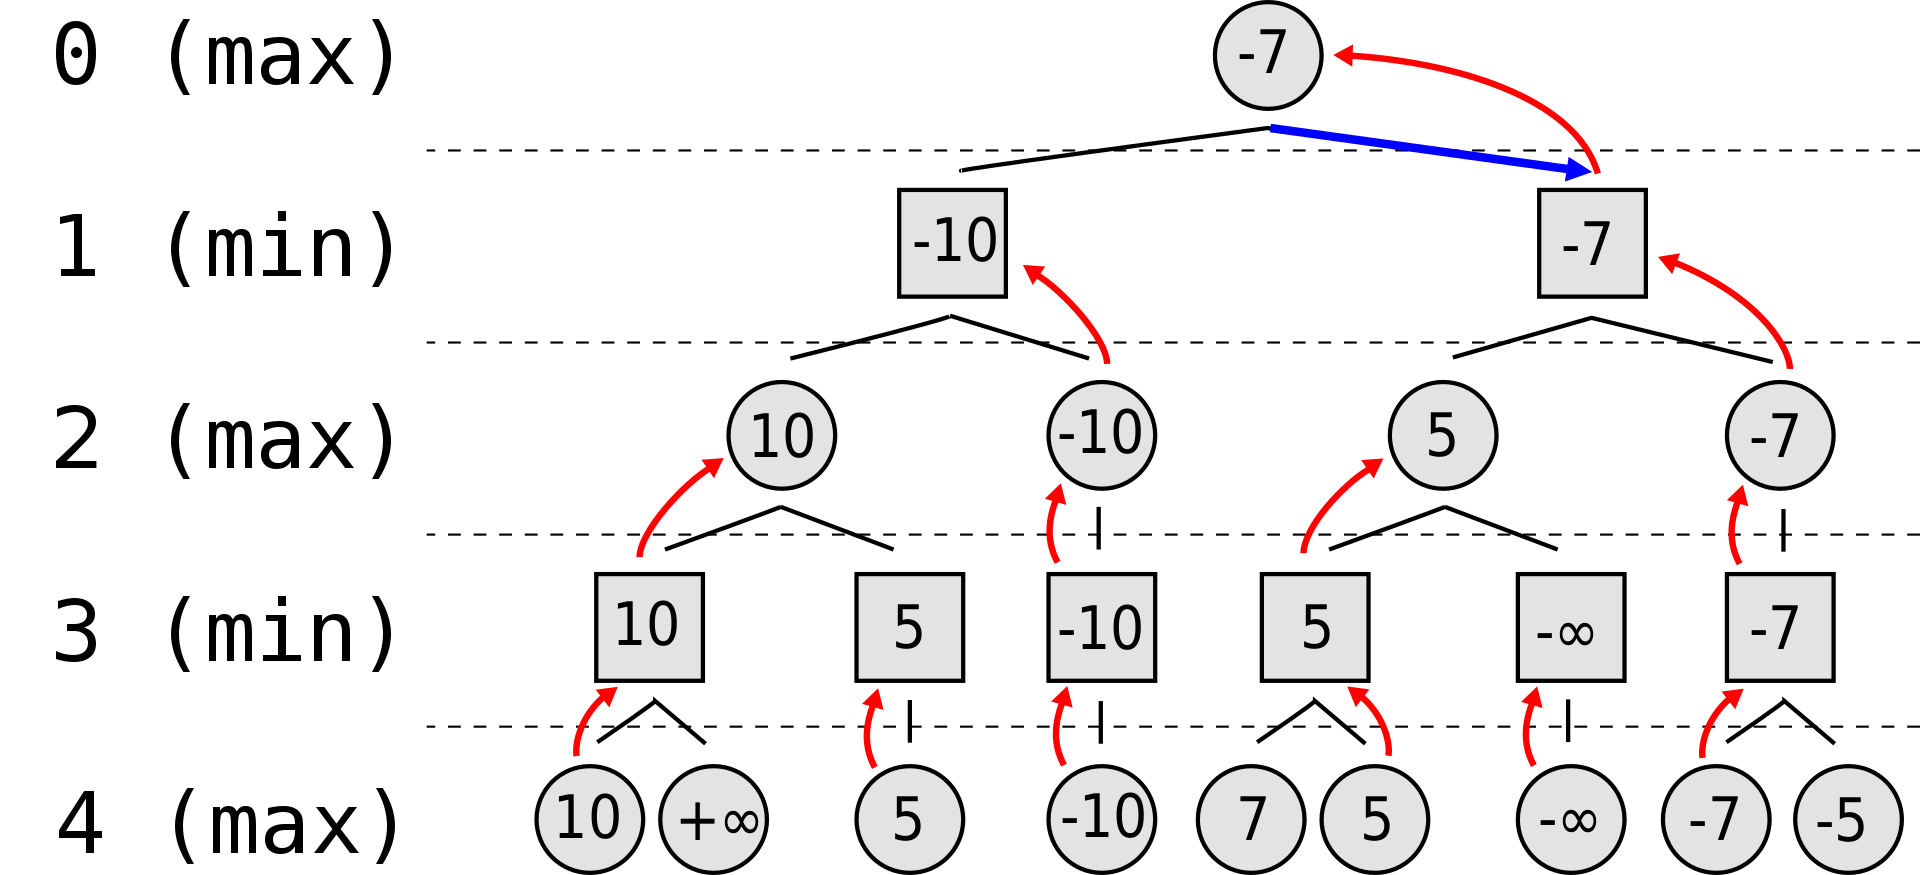
\includegraphics[width=0.4\textwidth]{images/minimax_tree.png}
    \caption{Minimax game tree visualization}
    \label{fig:minimax_tree}
\end{figure}

In Figure \ref{fig:minimax_tree}, the terminal nodes at the bottom represent the static evaluation of possible outcomes. These values are then propagated up to the root. At square nodes, the minimizing player selects the lowest available value. At circular nodes, the maximizing player selects the highest. The root node ultimately evaluates to -7, indicating the best achievable outcome under optimal play. 
The pseudocode for minimax is shown below:
\begin{verbatim}
function minimax(n, d, maxPlayer):
    if d == 0 or n is terminal:
        return evaluation(n)

    if maxPlayer:
        // Infinite negative value
        value = -10000 
        for each child of n:
            value = max(value, 
                minimax(child, d - 1, False)
            )
        return value
    else:
        // Infinite positive value
        value = +10000

        for each child of n:
            value = min(value, 
                minimax(child, d - 1, True)
            )
        return value
end function
\end{verbatim}

\subsection{Negamax}
The negamax algorithm takes advantage of the symmetry between maximizing and minimizing players. 
Instead of alternating between maximizing and minimizing the score at each level, it expresses both players with a single change of evaluation sign at each level. 
Formally, while minimax requires two cases (see Equation~\eqref{eq:minimax}):

\vspace{1em}

\resizebox{0.9\linewidth}{!}{%
    $\text{minimax}(s) = 
    \begin{cases}
        \text{eval}(s) & \text{if terminal} \\
        \max_{a \in A(s)} \text{minimax}(R(s, a)) & \text{if } p = \text{MAX} \\
        \min_{a \in A(s)} \text{minimax}(R(s, a)) & \text{if } p = \text{MIN}
    \end{cases}$
    \label{eq:minimax}
}

\vspace{1em}

Negamax rewrites the problem as:

\vspace{1em}

\resizebox{0.9\linewidth}{!}{%
    $\text{negamax}(s) = 
    \begin{cases}
        \text{eval}(s) & \text{if terminal} \\
        \max_{a \in A(s)} -\text{negamax}(R(s, a)) & \text{otherwise}
    \end{cases}$
    \label{eq:negamax}
}

\vspace{1em}

Where:
\begin{itemize}
    \item $s$ is the current game state
    \item $\text{A}(s)$ is the set of possible moves from state $s$
    \item $\text{R}(s, a)$ is the state resulting from taking action $a$ in state $s$
    \item $\text{p}(s)$ is the player whose turn it is in state $s$
    \item $\text{eval}(s)$ is the static evaluation function for state $s$
\end{itemize}.

Thus, as shown in Equation~\eqref{eq:negamax}, Negamax collapses the Minimax logic into a single recursive case with the advantage of shorter and cleaner implementations. 
The pseudocode for negamax is shown below:

\begin{verbatim}
function negamax(s, d):
    if d == 0 or s is terminal:
        return evaluation(s)

    // Infinite negative value
    value = -10000
    for each child of s:
        value = max(value, 
            negamax(child, d - 1)
        )
    return value
end function
\end{verbatim}
\subsection{Optimizations}

While Negamax simplifies the code, both Minimax and Negamax still suffer from exponential growth in the number of states explored. Optimizations aim to reduce the search space while preserving correctness or to trade off accuracy for speed.

\subsubsection{Alpha-Beta Pruning}
Alpha-Beta pruning enhances the Negamax (or Minimax) search by introducing two bounds, 
$\alpha$ (the best value that the maximizing player can guarantee) and $\beta$ (the best value that the minimizing player can guarantee). 
Whenever it is determined that a branch cannot possibly influence the final decision, that branch is discarded. 

\subsubsection{Move Ordering}
The effectiveness of Alpha-Beta pruning is highly dependent on the order in which moves are evaluated. 
If the most promising moves are examined first, the number of pruned branches increases, 
bringing the search closer to its optimal complexity. 
Heuristics such as capturing moves first in chess, or domain-specific evaluations, are often employed to improve ordering.

\subsubsection{Transposition Tables}
In many games, the same state can be reached through different sequences of moves. 
A transposition table is a cache that stores previously computed evaluations of game states. 
When the algorithm encounters a repeated position, it retrieves the stored value instead of recalculating the subtree, 
thereby saving computation time at the expense of additional memory.

\subsubsection{Iterative Deepening}
Iterative deepening performs a sequence of depth-limited searches, starting with depth one and progressively increasing. 
This approach has two key advantages: 
(1) it provides an approximate result if the search is interrupted, 
and (2) it generates information about promising moves at shallow depths, 
which can then be used to improve move ordering at deeper levels. 

\subsubsection{Comparison}
The Table~\ref{tab:negamax_optimizations} summarizes key optimizations applied to the Negamax algorithm. 

\begin{table}[h!]
    \centering
    \small
    \setlength{\tabcolsep}{3pt}
    \renewcommand{\arraystretch}{1.1}
    \caption{Comparison of Negamax Optimizations}
    \label{tab:negamax_optimizations}
    \begin{tabular}{|p{2.5cm}|p{4cm}|c|c|}
    \hline
    \textbf{Optimization} & \textbf{Description} & \textbf{Best} & \textbf{Worst} \\ \hline
    Alpha-Beta & Prunes irrelevant branches & $O(b^{d/2})$ & $O(b^d)$ \\ \hline
    Move Ordering & Prioritizes strong moves first & $O(b^{d/2})$ & $O(b^d)$ \\ \hline
    Transposition & Caches computed states & $O(b^{d/2})$ & $O(b^d)$ \\ \hline
    Iterative Deepening & Progressive depth search & $O(b^d)$ & $O(b^d)$ \\ \hline
    \end{tabular}
\end{table}

\section{Applications}

The Negamax algorithm, as a reformulation of Minimax, has been widely applied in the development of 
two-player zero-sum games and adversarial search problems. Its ability to systematically evaluate 
game states makes it fundamental in both academic study and real-world implementations.

\begin{itemize}
    \item \textbf{Classical Board Games:} 
    \begin{itemize}
        \item Forms the basis of AI agents for chess, checkers, tic-tac-toe, Othello, and Go (with depth limitations). 
        \item When combined with Alpha-Beta pruning and heuristic evaluation functions, it allows competitive play against human opponents.
    \end{itemize}

    \item \textbf{Computer and Video Games:} 
    \begin{itemize}
        \item Used for AI decision-making in strategy games with two players or opposing factions \cite{viazovskyi2018staralgo}.
        \item Provides a predictable and explainable decision process that can be enhanced with domain-specific heuristics.
    \end{itemize}

    \item \textbf{Research and Education:} 
    \begin{itemize}
        \item Widely used to teach concepts of game theory, artificial intelligence, and algorithm design.
        \item Its simple recursive formulation illustrates adversarial search, heuristic evaluation, and the impact of optimizations such as pruning.
    \end{itemize}

    \item \textbf{Beyond Games:} 
    \begin{itemize}
        \item Principles have been extended to other zero-sum decision-making scenarios \cite{ai2020nonneural}.
        \item Examples include economic simulations, resource allocation problems, and simplified models of negotiation.
    \end{itemize}
\end{itemize}


\bibliographystyle{plain}   
\bibliography{references}   


\end{document}